\documentclass[1p]{elsarticle_modified}
%\bibliographystyle{elsarticle-num}

%\usepackage[colorlinks]{hyperref}
%\usepackage{abbrmath_seonhwa} %\Abb, \Ascr, \Acal ,\Abf, \Afrak
\usepackage{amsfonts}
\usepackage{amssymb}
\usepackage{amsmath}
\usepackage{amsthm}
\usepackage{scalefnt}
\usepackage{amsbsy}
\usepackage{kotex}
\usepackage{caption}
\usepackage{subfig}
\usepackage{color}
\usepackage{graphicx}
\usepackage{xcolor} %% white, black, red, green, blue, cyan, magenta, yellow
\usepackage{float}
\usepackage{setspace}
\usepackage{hyperref}

\usepackage{tikz}
\usetikzlibrary{arrows}

\usepackage{multirow}
\usepackage{array} % fixed length table
\usepackage{hhline}

%%%%%%%%%%%%%%%%%%%%%
\makeatletter
\renewcommand*\env@matrix[1][\arraystretch]{%
	\edef\arraystretch{#1}%
	\hskip -\arraycolsep
	\let\@ifnextchar\new@ifnextchar
	\array{*\c@MaxMatrixCols c}}
\makeatother %https://tex.stackexchange.com/questions/14071/how-can-i-increase-the-line-spacing-in-a-matrix
%%%%%%%%%%%%%%%

\usepackage[normalem]{ulem}

\newcommand{\msout}[1]{\ifmmode\text{\sout{\ensuremath{#1}}}\else\sout{#1}\fi}
%SOURCE: \msout is \stkout macro in https://tex.stackexchange.com/questions/20609/strikeout-in-math-mode

\newcommand{\cancel}[1]{
	\ifmmode
	{\color{red}\msout{#1}}
	\else
	{\color{red}\sout{#1}}
	\fi
}

\newcommand{\add}[1]{
	{\color{blue}\uwave{#1}}
}

\newcommand{\replace}[2]{
	\ifmmode
	{\color{red}\msout{#1}}{\color{blue}\uwave{#2}}
	\else
	{\color{red}\sout{#1}}{\color{blue}\uwave{#2}}
	\fi
}

\newcommand{\Sol}{\mathcal{S}} %segment
\newcommand{\D}{D} %diagram
\newcommand{\A}{\mathcal{A}} %arc


%%%%%%%%%%%%%%%%%%%%%%%%%%%%%5 test

\def\sl{\operatorname{\textup{SL}}(2,\Cbb)}
\def\psl{\operatorname{\textup{PSL}}(2,\Cbb)}
\def\quan{\mkern 1mu \triangleright \mkern 1mu}

\theoremstyle{definition}
\newtheorem{thm}{Theorem}[section]
\newtheorem{prop}[thm]{Proposition}
\newtheorem{lem}[thm]{Lemma}
\newtheorem{ques}[thm]{Question}
\newtheorem{cor}[thm]{Corollary}
\newtheorem{defn}[thm]{Definition}
\newtheorem{exam}[thm]{Example}
\newtheorem{rmk}[thm]{Remark}
\newtheorem{alg}[thm]{Algorithm}

\newcommand{\I}{\sqrt{-1}}
\begin{document}

%\begin{frontmatter}
%
%\title{Boundary parabolic representations of knots up to 8 crossings}
%
%%% Group authors per affiliation:
%\author{Yunhi Cho} 
%\address{Department of Mathematics, University of Seoul, Seoul, Korea}
%\ead{yhcho@uos.ac.kr}
%
%
%\author{Seonhwa Kim} %\fnref{s_kim}}
%\address{Center for Geometry and Physics, Institute for Basic Science, Pohang, 37673, Korea}
%\ead{ryeona17@ibs.re.kr}
%
%\author{Hyuk Kim}
%\address{Department of Mathematical Sciences, Seoul National University, Seoul 08826, Korea}
%\ead{hyukkim@snu.ac.kr}
%
%\author{Seokbeom Yoon}
%\address{Department of Mathematical Sciences, Seoul National University, Seoul, 08826,  Korea}
%\ead{sbyoon15@snu.ac.kr}
%
%\begin{abstract}
%We find all boundary parabolic representation of knots up to 8 crossings.
%
%\end{abstract}
%\begin{keyword}
%    \MSC[2010] 57M25 
%\end{keyword}
%
%\end{frontmatter}

%\linenumbers
%\tableofcontents
%
\newcommand\colored[1]{\textcolor{white}{\rule[-0.35ex]{0.8em}{1.4ex}}\kern-0.8em\color{red} #1}%
%\newcommand\colored[1]{\textcolor{white}{ #1}\kern-2.17ex	\textcolor{white}{ #1}\kern-1.81ex	\textcolor{white}{ #1}\kern-2.15ex\color{red}#1	}

{\Large $\underline{12a_{0787}~(K12a_{0787})}$}

\setlength{\tabcolsep}{10pt}
\renewcommand{\arraystretch}{1.6}
\vspace{1cm}\begin{tabular}{m{100pt}>{\centering\arraybackslash}m{274pt}}
\multirow{5}{120pt}{
	\centering
	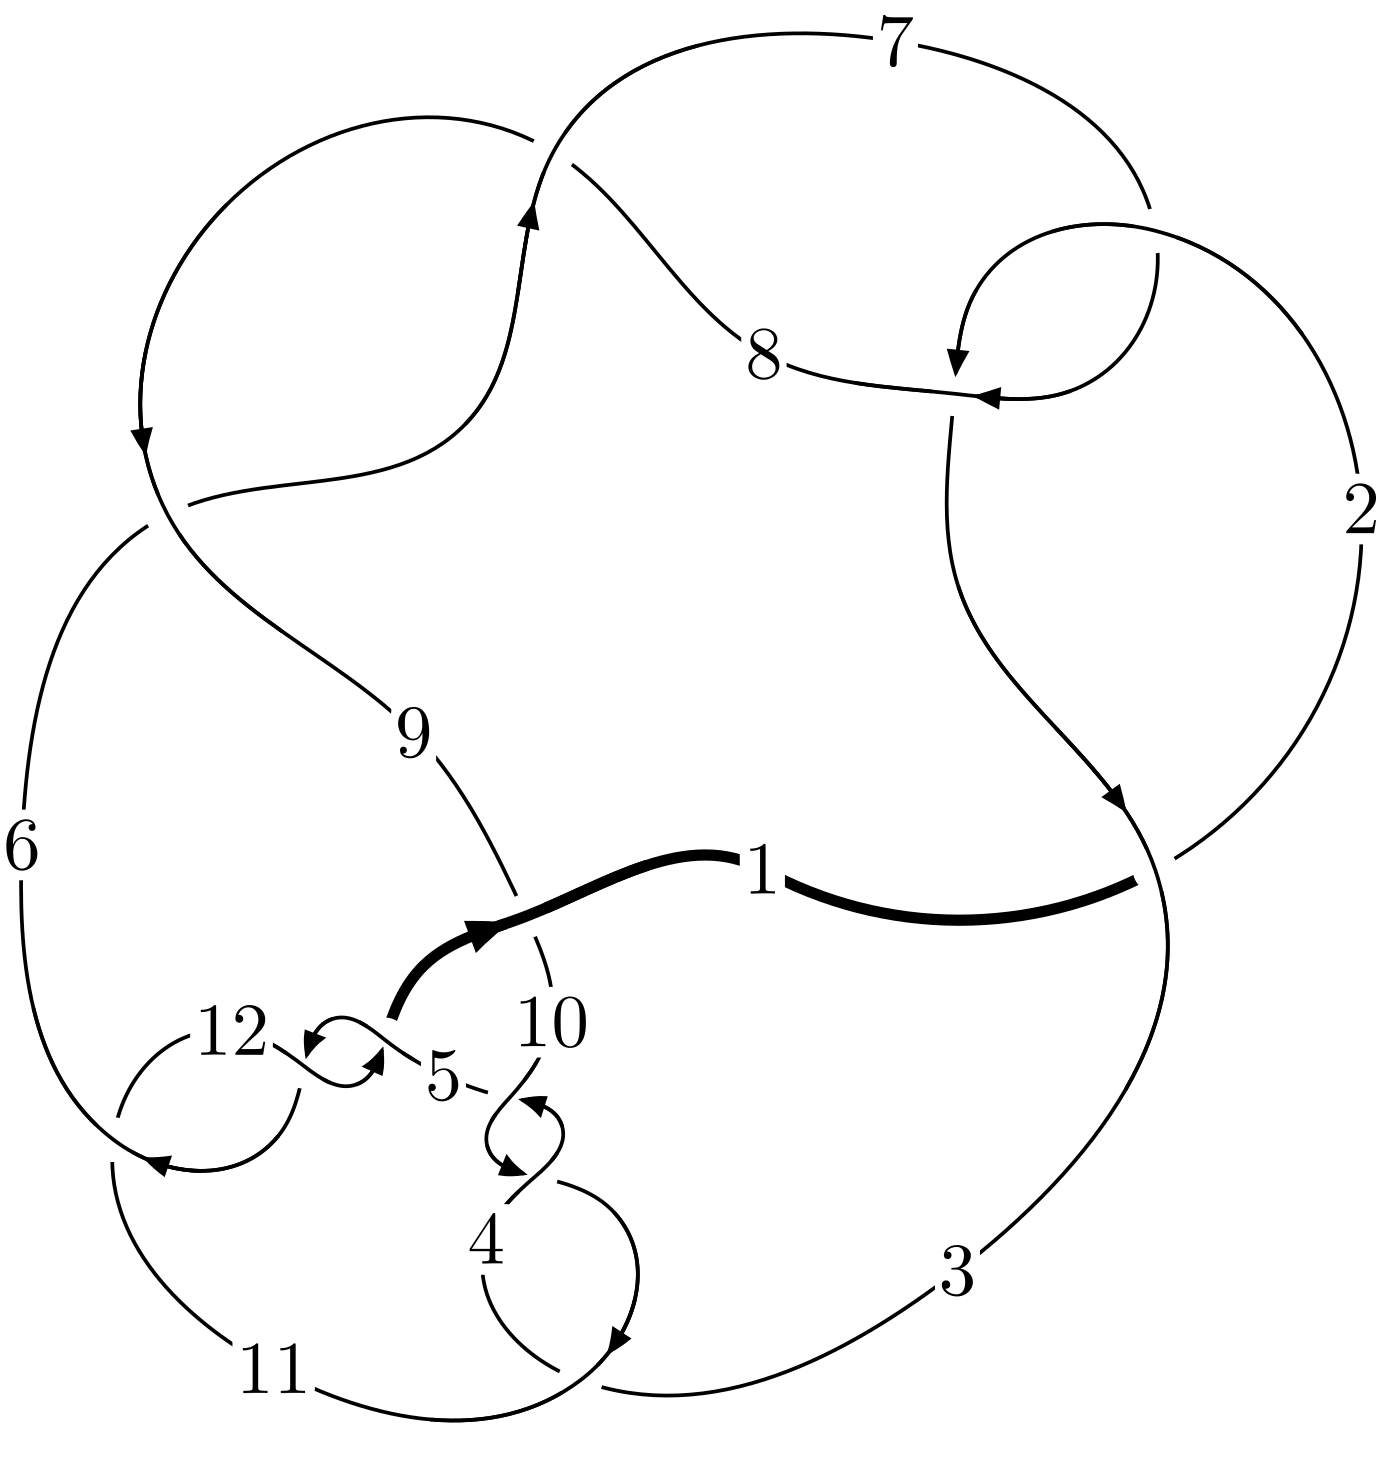
\includegraphics[width=112pt]{../../../GIT/diagram.site/Diagrams/png/1588_12a_0787.png}\\
\ \ \ A knot diagram\footnotemark}&
\allowdisplaybreaks
\textbf{Linearized knot diagam} \\
\cline{2-2}
 &
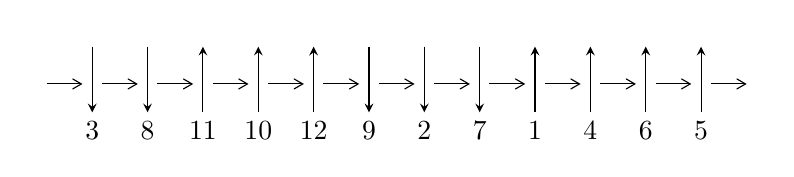
\begin{tikzpicture}[x=20pt, y=17pt]
	% nodes
	\node (C0) at (0, 0) {};
	\node (C1) at (1, 0) {};
	\node (C1U) at (1, +1) {};
	\node (C1D) at (1, -1) {3};

	\node (C2) at (2, 0) {};
	\node (C2U) at (2, +1) {};
	\node (C2D) at (2, -1) {8};

	\node (C3) at (3, 0) {};
	\node (C3U) at (3, +1) {};
	\node (C3D) at (3, -1) {11};

	\node (C4) at (4, 0) {};
	\node (C4U) at (4, +1) {};
	\node (C4D) at (4, -1) {10};

	\node (C5) at (5, 0) {};
	\node (C5U) at (5, +1) {};
	\node (C5D) at (5, -1) {12};

	\node (C6) at (6, 0) {};
	\node (C6U) at (6, +1) {};
	\node (C6D) at (6, -1) {9};

	\node (C7) at (7, 0) {};
	\node (C7U) at (7, +1) {};
	\node (C7D) at (7, -1) {2};

	\node (C8) at (8, 0) {};
	\node (C8U) at (8, +1) {};
	\node (C8D) at (8, -1) {7};

	\node (C9) at (9, 0) {};
	\node (C9U) at (9, +1) {};
	\node (C9D) at (9, -1) {1};

	\node (C10) at (10, 0) {};
	\node (C10U) at (10, +1) {};
	\node (C10D) at (10, -1) {4};

	\node (C11) at (11, 0) {};
	\node (C11U) at (11, +1) {};
	\node (C11D) at (11, -1) {6};

	\node (C12) at (12, 0) {};
	\node (C12U) at (12, +1) {};
	\node (C12D) at (12, -1) {5};
	\node (C13) at (13, 0) {};

	% arrows
	\draw[->,>={angle 60}]
	(C0) edge (C1) (C1) edge (C2) (C2) edge (C3) (C3) edge (C4) (C4) edge (C5) (C5) edge (C6) (C6) edge (C7) (C7) edge (C8) (C8) edge (C9) (C9) edge (C10) (C10) edge (C11) (C11) edge (C12) (C12) edge (C13) ;	\draw[->,>=stealth]
	(C1U) edge (C1D) (C2U) edge (C2D) (C3D) edge (C3U) (C4D) edge (C4U) (C5D) edge (C5U) (C6U) edge (C6D) (C7U) edge (C7D) (C8U) edge (C8D) (C9D) edge (C9U) (C10D) edge (C10U) (C11D) edge (C11U) (C12D) edge (C12U) ;
	\end{tikzpicture} \\
\hhline{~~} \\& 
\textbf{Solving Sequence} \\ \cline{2-2} 
 &
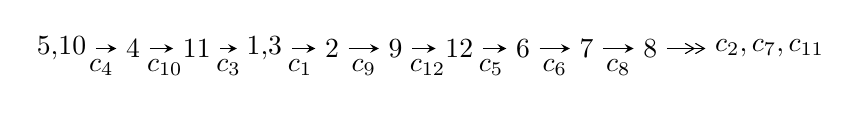
\begin{tikzpicture}[x=23pt, y=7pt]
	% node
	\node (A0) at (-1/8, 0) {5,10};
	\node (A1) at (1, 0) {4};
	\node (A2) at (2, 0) {11};
	\node (A3) at (49/16, 0) {1,3};
	\node (A4) at (33/8, 0) {2};
	\node (A5) at (41/8, 0) {9};
	\node (A6) at (49/8, 0) {12};
	\node (A7) at (57/8, 0) {6};
	\node (A8) at (65/8, 0) {7};
	\node (A9) at (73/8, 0) {8};
	\node (C1) at (1/2, -1) {$c_{4}$};
	\node (C2) at (3/2, -1) {$c_{10}$};
	\node (C3) at (5/2, -1) {$c_{3}$};
	\node (C4) at (29/8, -1) {$c_{1}$};
	\node (C5) at (37/8, -1) {$c_{9}$};
	\node (C6) at (45/8, -1) {$c_{12}$};
	\node (C7) at (53/8, -1) {$c_{5}$};
	\node (C8) at (61/8, -1) {$c_{6}$};
	\node (C9) at (69/8, -1) {$c_{8}$};
	\node (A10) at (11, 0) {$c_{2},c_{7},c_{11}$};

	% edge
	\draw[->,>=stealth]	
	(A0) edge (A1) (A1) edge (A2) (A2) edge (A3) (A3) edge (A4) (A4) edge (A5) (A5) edge (A6) (A6) edge (A7) (A7) edge (A8) (A8) edge (A9) ;
	\draw[->>,>={angle 60}]	
	(A9) edge (A10);
\end{tikzpicture} \\ 

\end{tabular} \\

\footnotetext{
The image of knot diagram is generated by the software ``\textbf{Draw programme}" developed by Andrew Bartholomew(\url{http://www.layer8.co.uk/maths/draw/index.htm\#Running-draw}), where we modified some parts for our purpose(\url{https://github.com/CATsTAILs/LinksPainter}).
}\phantom \\ \newline 
\centering \textbf{Ideals for irreducible components\footnotemark of $X_{\text{par}}$} 
 
\begin{align*}
I^u_{1}&=\langle 
b- u,\;u^{27}+u^{26}+\cdots+16 a+1,\;u^{28}+17 u^{26}+\cdots- u+1\rangle \\
I^u_{2}&=\langle 
-2521899524065 u^{37}-1276991146481 u^{36}+\cdots+13233245626882 b+40729676197632,\\
\phantom{I^u_{2}}&\phantom{= \langle  }-9138522337506 u^{37}-7893613959922 u^{36}+\cdots+13233245626882 a+87046035891719,\\
\phantom{I^u_{2}}&\phantom{= \langle  }u^{38}+u^{37}+\cdots-7 u+2\rangle \\
I^u_{3}&=\langle 
b+u,\;a^4+a^3+3 a^2+2 a+1,\;u^2+1\rangle \\
\\
\end{align*}
\raggedright * 3 irreducible components of $\dim_{\mathbb{C}}=0$, with total 74 representations.\\
\footnotetext{All coefficients of polynomials are rational numbers. But the coefficients are sometimes approximated in decimal forms when there is not enough margin.}
\newpage
\renewcommand{\arraystretch}{1}
\centering \section*{I. $I^u_{1}= \langle b- u,\;u^{27}+u^{26}+\cdots+16 a+1,\;u^{28}+17 u^{26}+\cdots- u+1 \rangle$}
\flushleft \textbf{(i) Arc colorings}\\
\begin{tabular}{m{7pt} m{180pt} m{7pt} m{180pt} }
\flushright $a_{5}=$&$\begin{pmatrix}1\\0\end{pmatrix}$ \\
\flushright $a_{10}=$&$\begin{pmatrix}0\\u\end{pmatrix}$ \\
\flushright $a_{4}=$&$\begin{pmatrix}1\\u^2\end{pmatrix}$ \\
\flushright $a_{11}=$&$\begin{pmatrix}u\\u^3+u\end{pmatrix}$ \\
\flushright $a_{1}=$&$\begin{pmatrix}-\frac{1}{16} u^{27}-\frac{1}{16} u^{26}+\cdots+3 u-\frac{1}{16}\\u\end{pmatrix}$ \\
\flushright $a_{3}=$&$\begin{pmatrix}u^2+1\\u^4+2 u^2\end{pmatrix}$ \\
\flushright $a_{2}=$&$\begin{pmatrix}-\frac{1}{16} u^{27}-\frac{1}{16} u^{26}+\cdots+2 u-\frac{1}{16}\\-\frac{1}{16} u^{27}-\frac{1}{16} u^{26}+\cdots+u-\frac{1}{16}\end{pmatrix}$ \\
\flushright $a_{9}=$&$\begin{pmatrix}-\frac{1}{8} u^{25}-\frac{1}{8} u^{24}+\cdots-\frac{87}{8} u^3-\frac{1}{8}\\-\frac{1}{16} u^{27}-\frac{1}{16} u^{26}+\cdots+u-\frac{1}{16}\end{pmatrix}$ \\
\flushright $a_{12}=$&$\begin{pmatrix}-\frac{1}{16} u^{27}-\frac{1}{16} u^{26}+\cdots+2 u-\frac{1}{16}\\u\end{pmatrix}$ \\
\flushright $a_{6}=$&$\begin{pmatrix}\frac{1}{16} u^{27}-\frac{1}{16} u^{26}+\cdots+\frac{1}{8} u+\frac{15}{16}\\- u^2\end{pmatrix}$ \\
\flushright $a_{7}=$&$\begin{pmatrix}-0.687500 u^{27}+0.437500 u^{26}+\cdots-1.62500 u+1.56250\\-\frac{1}{16} u^{27}-\frac{1}{16} u^{26}+\cdots-\frac{1}{4} u+\frac{1}{16}\end{pmatrix}$ \\
\flushright $a_{8}=$&$\begin{pmatrix}-0.187500 u^{27}+0.187500 u^{26}+\cdots+0.375000 u+1.31250\\\frac{1}{4} u^{27}+\frac{3}{8} u^{26}+\cdots+\frac{7}{8} u+\frac{5}{8}\end{pmatrix}$\\&\end{tabular}
\flushleft \textbf{(ii) Obstruction class $= -1$}\\~\\
\flushleft \textbf{(iii) Cusp Shapes $= \frac{11}{4} u^{27}-\frac{1}{4} u^{26}+\cdots-\frac{9}{2} u-3$}\\~\\
\newpage\renewcommand{\arraystretch}{1}
\flushleft \textbf{(iv) u-Polynomials at the component}\newline \\
\begin{tabular}{m{50pt}|m{274pt}}
Crossings & \hspace{64pt}u-Polynomials at each crossing \\
\hline $$\begin{aligned}c_{1},c_{6},c_{8}\end{aligned}$$&$\begin{aligned}
&u^{28}+7 u^{27}+\cdots+9 u+4
\end{aligned}$\\
\hline $$\begin{aligned}c_{2},c_{7}\end{aligned}$$&$\begin{aligned}
&u^{28}+3 u^{27}+\cdots- u+2
\end{aligned}$\\
\hline $$\begin{aligned}c_{3},c_{4},c_{5}\\c_{10},c_{11},c_{12}\end{aligned}$$&$\begin{aligned}
&u^{28}+17 u^{26}+\cdots+u+1
\end{aligned}$\\
\hline $$\begin{aligned}c_{9}\end{aligned}$$&$\begin{aligned}
&u^{28}-21 u^{27}+\cdots-24293 u+2642
\end{aligned}$\\
\hline
\end{tabular}\\~\\
\newpage\renewcommand{\arraystretch}{1}
\flushleft \textbf{(v) Riley Polynomials at the component}\newline \\
\begin{tabular}{m{50pt}|m{274pt}}
Crossings & \hspace{64pt}Riley Polynomials at each crossing \\
\hline $$\begin{aligned}c_{1},c_{6},c_{8}\end{aligned}$$&$\begin{aligned}
&y^{28}+29 y^{27}+\cdots+383 y+16
\end{aligned}$\\
\hline $$\begin{aligned}c_{2},c_{7}\end{aligned}$$&$\begin{aligned}
&y^{28}-7 y^{27}+\cdots-9 y+4
\end{aligned}$\\
\hline $$\begin{aligned}c_{3},c_{4},c_{5}\\c_{10},c_{11},c_{12}\end{aligned}$$&$\begin{aligned}
&y^{28}+34 y^{27}+\cdots+5 y+1
\end{aligned}$\\
\hline $$\begin{aligned}c_{9}\end{aligned}$$&$\begin{aligned}
&y^{28}+y^{27}+\cdots+72951 y+6980164
\end{aligned}$\\
\hline
\end{tabular}\\~\\
\newpage\flushleft \textbf{(vi) Complex Volumes and Cusp Shapes}
$$\begin{array}{c|c|c}  
\text{Solutions to }I^u_{1}& \I (\text{vol} + \sqrt{-1}CS) & \text{Cusp shape}\\
 \hline 
\begin{aligned}
u &= \phantom{-}0.668490 + 0.320146 I \\
a &= \phantom{-}1.70913 + 0.46510 I \\
b &= \phantom{-}0.668490 + 0.320146 I\end{aligned}
 & \phantom{-}6.28423 + 6.57769 I & \phantom{-}6.41221 - 7.42471 I \\ \hline\begin{aligned}
u &= \phantom{-}0.668490 - 0.320146 I \\
a &= \phantom{-}1.70913 - 0.46510 I \\
b &= \phantom{-}0.668490 - 0.320146 I\end{aligned}
 & \phantom{-}6.28423 - 6.57769 I & \phantom{-}6.41221 + 7.42471 I \\ \hline\begin{aligned}
u &= -0.675753 + 0.283618 I \\
a &= -1.69364 + 0.41228 I \\
b &= -0.675753 + 0.283618 I\end{aligned}
 & \phantom{-}6.57383 - 0.38638 I & \phantom{-}7.28743 + 2.11062 I \\ \hline\begin{aligned}
u &= -0.675753 - 0.283618 I \\
a &= -1.69364 - 0.41228 I \\
b &= -0.675753 - 0.283618 I\end{aligned}
 & \phantom{-}6.57383 + 0.38638 I & \phantom{-}7.28743 - 2.11062 I \\ \hline\begin{aligned}
u &= \phantom{-}0.010002 + 1.361850 I \\
a &= \phantom{-}0.08812 - 1.82299 I \\
b &= \phantom{-}0.010002 + 1.361850 I\end{aligned}
 & \phantom{-}0.98241 + 3.28877 I & -2.28562 - 2.49826 I \\ \hline\begin{aligned}
u &= \phantom{-}0.010002 - 1.361850 I \\
a &= \phantom{-}0.08812 + 1.82299 I \\
b &= \phantom{-}0.010002 - 1.361850 I\end{aligned}
 & \phantom{-}0.98241 - 3.28877 I & -2.28562 + 2.49826 I \\ \hline\begin{aligned}
u &= \phantom{-}0.479155 + 0.323957 I \\
a &= \phantom{-}1.41870 + 0.64071 I \\
b &= \phantom{-}0.479155 + 0.323957 I\end{aligned}
 & -0.70246 + 3.29244 I & \phantom{-}1.36299 - 9.65780 I \\ \hline\begin{aligned}
u &= \phantom{-}0.479155 - 0.323957 I \\
a &= \phantom{-}1.41870 - 0.64071 I \\
b &= \phantom{-}0.479155 - 0.323957 I\end{aligned}
 & -0.70246 - 3.29244 I & \phantom{-}1.36299 + 9.65780 I \\ \hline\begin{aligned}
u &= \phantom{-}0.018495 + 0.555616 I \\
a &= \phantom{-}0.11963 + 2.15929 I \\
b &= \phantom{-}0.018495 + 0.555616 I\end{aligned}
 & \phantom{-}5.02040 - 3.10627 I & \phantom{-}5.07926 + 2.30848 I \\ \hline\begin{aligned}
u &= \phantom{-}0.018495 - 0.555616 I \\
a &= \phantom{-}0.11963 - 2.15929 I \\
b &= \phantom{-}0.018495 - 0.555616 I\end{aligned}
 & \phantom{-}5.02040 + 3.10627 I & \phantom{-}5.07926 - 2.30848 I\\
 \hline 
 \end{array}$$\newpage$$\begin{array}{c|c|c}  
\text{Solutions to }I^u_{1}& \I (\text{vol} + \sqrt{-1}CS) & \text{Cusp shape}\\
 \hline 
\begin{aligned}
u &= \phantom{-}0.12806 + 1.49665 I \\
a &= \phantom{-}0.635356 - 0.790802 I \\
b &= \phantom{-}0.12806 + 1.49665 I\end{aligned}
 & -8.20165 + 3.12776 I & -1.78341 - 2.86928 I \\ \hline\begin{aligned}
u &= \phantom{-}0.12806 - 1.49665 I \\
a &= \phantom{-}0.635356 + 0.790802 I \\
b &= \phantom{-}0.12806 - 1.49665 I\end{aligned}
 & -8.20165 - 3.12776 I & -1.78341 + 2.86928 I \\ \hline\begin{aligned}
u &= -0.467343 + 0.123789 I \\
a &= -1.256740 + 0.253657 I \\
b &= -0.467343 + 0.123789 I\end{aligned}
 & \phantom{-}0.942412 - 0.321823 I & \phantom{-}9.93783 + 1.87531 I \\ \hline\begin{aligned}
u &= -0.467343 - 0.123789 I \\
a &= -1.256740 - 0.253657 I \\
b &= -0.467343 - 0.123789 I\end{aligned}
 & \phantom{-}0.942412 + 0.321823 I & \phantom{-}9.93783 - 1.87531 I \\ \hline\begin{aligned}
u &= \phantom{-}0.33592 + 1.48906 I \\
a &= \phantom{-}1.343430 - 0.294813 I \\
b &= \phantom{-}0.33592 + 1.48906 I\end{aligned}
 & -4.85757 + 8.12866 I & -0.65039 - 3.19597 I \\ \hline\begin{aligned}
u &= \phantom{-}0.33592 - 1.48906 I \\
a &= \phantom{-}1.343430 + 0.294813 I \\
b &= \phantom{-}0.33592 - 1.48906 I\end{aligned}
 & -4.85757 - 8.12866 I & -0.65039 + 3.19597 I \\ \hline\begin{aligned}
u &= \phantom{-}0.24720 + 1.51029 I \\
a &= \phantom{-}1.054950 - 0.471434 I \\
b &= \phantom{-}0.24720 + 1.51029 I\end{aligned}
 & -10.29860 + 5.81281 I & -1.13573 - 2.99582 I \\ \hline\begin{aligned}
u &= \phantom{-}0.24720 - 1.51029 I \\
a &= \phantom{-}1.054950 + 0.471434 I \\
b &= \phantom{-}0.24720 - 1.51029 I\end{aligned}
 & -10.29860 - 5.81281 I & -1.13573 + 2.99582 I \\ \hline\begin{aligned}
u &= -0.34687 + 1.50237 I \\
a &= -1.331920 - 0.237656 I \\
b &= -0.34687 + 1.50237 I\end{aligned}
 & -5.4858 - 14.4431 I & -1.57414 + 7.85260 I \\ \hline\begin{aligned}
u &= -0.34687 - 1.50237 I \\
a &= -1.331920 + 0.237656 I \\
b &= -0.34687 - 1.50237 I\end{aligned}
 & -5.4858 + 14.4431 I & -1.57414 - 7.85260 I\\
 \hline 
 \end{array}$$\newpage$$\begin{array}{c|c|c}  
\text{Solutions to }I^u_{1}& \I (\text{vol} + \sqrt{-1}CS) & \text{Cusp shape}\\
 \hline 
\begin{aligned}
u &= -0.09545 + 1.55729 I \\
a &= -0.408600 - 0.576483 I \\
b &= -0.09545 + 1.55729 I\end{aligned}
 & -9.25929 + 2.16393 I & -3.88367 - 2.85288 I \\ \hline\begin{aligned}
u &= -0.09545 - 1.55729 I \\
a &= -0.408600 + 0.576483 I \\
b &= -0.09545 - 1.55729 I\end{aligned}
 & -9.25929 - 2.16393 I & -3.88367 + 2.85288 I \\ \hline\begin{aligned}
u &= -0.28719 + 1.53991 I \\
a &= -1.099080 - 0.292514 I \\
b &= -0.28719 + 1.53991 I\end{aligned}
 & -13.1202 - 9.6253 I & -6.14913 + 7.05980 I \\ \hline\begin{aligned}
u &= -0.28719 - 1.53991 I \\
a &= -1.099080 + 0.292514 I \\
b &= -0.28719 - 1.53991 I\end{aligned}
 & -13.1202 + 9.6253 I & -6.14913 - 7.05980 I \\ \hline\begin{aligned}
u &= -0.21010 + 1.56283 I \\
a &= -0.823988 - 0.384208 I \\
b &= -0.21010 + 1.56283 I\end{aligned}
 & -14.2962 - 3.2369 I & -8.20460 + 0. I\phantom{ +0.000000I} \\ \hline\begin{aligned}
u &= -0.21010 - 1.56283 I \\
a &= -0.823988 + 0.384208 I \\
b &= -0.21010 - 1.56283 I\end{aligned}
 & -14.2962 + 3.2369 I & -8.20460 + 0. I\phantom{ +0.000000I} \\ \hline\begin{aligned}
u &= \phantom{-}0.195378 + 0.368416 I \\
a &= \phantom{-}0.744647 + 1.097280 I \\
b &= \phantom{-}0.195378 + 0.368416 I\end{aligned}
 & -1.28464 - 0.85587 I & -2.41301 + 0.23823 I \\ \hline\begin{aligned}
u &= \phantom{-}0.195378 - 0.368416 I \\
a &= \phantom{-}0.744647 - 1.097280 I \\
b &= \phantom{-}0.195378 - 0.368416 I\end{aligned}
 & -1.28464 + 0.85587 I & -2.41301 - 0.23823 I\\
 \hline 
 \end{array}$$\newpage\newpage\renewcommand{\arraystretch}{1}
\centering \section*{II. $I^u_{2}= \langle -2.52\times10^{12} u^{37}-1.28\times10^{12} u^{36}+\cdots+1.32\times10^{13} b+4.07\times10^{13},\;-9.14\times10^{12} u^{37}-7.89\times10^{12} u^{36}+\cdots+1.32\times10^{13} a+8.70\times10^{13},\;u^{38}+u^{37}+\cdots-7 u+2 \rangle$}
\flushleft \textbf{(i) Arc colorings}\\
\begin{tabular}{m{7pt} m{180pt} m{7pt} m{180pt} }
\flushright $a_{5}=$&$\begin{pmatrix}1\\0\end{pmatrix}$ \\
\flushright $a_{10}=$&$\begin{pmatrix}0\\u\end{pmatrix}$ \\
\flushright $a_{4}=$&$\begin{pmatrix}1\\u^2\end{pmatrix}$ \\
\flushright $a_{11}=$&$\begin{pmatrix}u\\u^3+u\end{pmatrix}$ \\
\flushright $a_{1}=$&$\begin{pmatrix}0.690573 u^{37}+0.596499 u^{36}+\cdots+27.4552 u-6.57783\\0.190573 u^{37}+0.0964987 u^{36}+\cdots+7.95523 u-3.07783\end{pmatrix}$ \\
\flushright $a_{3}=$&$\begin{pmatrix}u^2+1\\u^4+2 u^2\end{pmatrix}$ \\
\flushright $a_{2}=$&$\begin{pmatrix}0.504054 u^{37}+0.688185 u^{36}+\cdots+16.6062 u-3.16265\\0.385043 u^{37}+0.407527 u^{36}+\cdots+10.1840 u-3.31197\end{pmatrix}$ \\
\flushright $a_{9}=$&$\begin{pmatrix}1.06524 u^{37}+0.963635 u^{36}+\cdots+35.3708 u-9.46751\\0.374672 u^{37}+0.367136 u^{36}+\cdots+8.91556 u-2.88968\end{pmatrix}$ \\
\flushright $a_{12}=$&$\begin{pmatrix}\frac{1}{2} u^{37}+\frac{1}{2} u^{36}+\cdots+\frac{39}{2} u-\frac{7}{2}\\0.190573 u^{37}+0.0964987 u^{36}+\cdots+7.95523 u-3.07783\end{pmatrix}$ \\
\flushright $a_{6}=$&$\begin{pmatrix}1.53891 u^{37}+1.72949 u^{36}+\cdots+25.2431 u-1.81717\\-0.0940743 u^{37}+0.0900246 u^{36}+\cdots-1.74382 u+0.618854\end{pmatrix}$ \\
\flushright $a_{7}=$&$\begin{pmatrix}-0.540566 u^{37}-0.819412 u^{36}+\cdots-5.62383 u-4.68707\\-0.203220 u^{37}-0.490174 u^{36}+\cdots-4.02159 u-2.26098\end{pmatrix}$ \\
\flushright $a_{8}=$&$\begin{pmatrix}-0.215007 u^{37}+0.108358 u^{36}+\cdots-9.07233 u+2.38121\\-0.203697 u^{37}-0.475149 u^{36}+\cdots-4.71463 u-1.10982\end{pmatrix}$\\&\end{tabular}
\flushleft \textbf{(ii) Obstruction class $= -1$}\\~\\
\flushleft \textbf{(iii) Cusp Shapes $= \frac{2578336863836}{6616622813441} u^{37}-\frac{917470771354}{6616622813441} u^{36}+\cdots+\frac{231718964327524}{6616622813441} u-\frac{47642846027518}{6616622813441}$}\\~\\
\newpage\renewcommand{\arraystretch}{1}
\flushleft \textbf{(iv) u-Polynomials at the component}\newline \\
\begin{tabular}{m{50pt}|m{274pt}}
Crossings & \hspace{64pt}u-Polynomials at each crossing \\
\hline $$\begin{aligned}c_{1},c_{6},c_{8}\end{aligned}$$&$\begin{aligned}
&(u^{19}+5 u^{18}+\cdots+2 u+1)^{2}
\end{aligned}$\\
\hline $$\begin{aligned}c_{2},c_{7}\end{aligned}$$&$\begin{aligned}
&(u^{19}- u^{18}+\cdots+u^2-1)^{2}
\end{aligned}$\\
\hline $$\begin{aligned}c_{3},c_{4},c_{5}\\c_{10},c_{11},c_{12}\end{aligned}$$&$\begin{aligned}
&u^{38}- u^{37}+\cdots+7 u+2
\end{aligned}$\\
\hline $$\begin{aligned}c_{9}\end{aligned}$$&$\begin{aligned}
&(u^{19}+7 u^{18}+\cdots+2 u-1)^{2}
\end{aligned}$\\
\hline
\end{tabular}\\~\\
\newpage\renewcommand{\arraystretch}{1}
\flushleft \textbf{(v) Riley Polynomials at the component}\newline \\
\begin{tabular}{m{50pt}|m{274pt}}
Crossings & \hspace{64pt}Riley Polynomials at each crossing \\
\hline $$\begin{aligned}c_{1},c_{6},c_{8}\end{aligned}$$&$\begin{aligned}
&(y^{19}+19 y^{18}+\cdots+10 y-1)^{2}
\end{aligned}$\\
\hline $$\begin{aligned}c_{2},c_{7}\end{aligned}$$&$\begin{aligned}
&(y^{19}-5 y^{18}+\cdots+2 y-1)^{2}
\end{aligned}$\\
\hline $$\begin{aligned}c_{3},c_{4},c_{5}\\c_{10},c_{11},c_{12}\end{aligned}$$&$\begin{aligned}
&y^{38}+31 y^{37}+\cdots+107 y+4
\end{aligned}$\\
\hline $$\begin{aligned}c_{9}\end{aligned}$$&$\begin{aligned}
&(y^{19}+11 y^{18}+\cdots+42 y-1)^{2}
\end{aligned}$\\
\hline
\end{tabular}\\~\\
\newpage\flushleft \textbf{(vi) Complex Volumes and Cusp Shapes}
$$\begin{array}{c|c|c}  
\text{Solutions to }I^u_{2}& \I (\text{vol} + \sqrt{-1}CS) & \text{Cusp shape}\\
 \hline 
\begin{aligned}
u &= -0.745217 + 0.660881 I \\
a &= \phantom{-}0.786897 - 0.760848 I \\
b &= \phantom{-}0.03575 - 1.42698 I\end{aligned}
 & -6.91199 + 0.16816 I & -6.16829 - 0.91431 I \\ \hline\begin{aligned}
u &= -0.745217 - 0.660881 I \\
a &= \phantom{-}0.786897 + 0.760848 I \\
b &= \phantom{-}0.03575 + 1.42698 I\end{aligned}
 & -6.91199 - 0.16816 I & -6.16829 + 0.91431 I \\ \hline\begin{aligned}
u &= -0.909367 + 0.387387 I \\
a &= \phantom{-}1.17340 - 1.04324 I \\
b &= \phantom{-}0.24265 - 1.43973 I\end{aligned}
 & \phantom{-}0.60648 - 9.88550 I & \phantom{-}1.13872 + 7.31129 I \\ \hline\begin{aligned}
u &= -0.909367 - 0.387387 I \\
a &= \phantom{-}1.17340 + 1.04324 I \\
b &= \phantom{-}0.24265 + 1.43973 I\end{aligned}
 & \phantom{-}0.60648 + 9.88550 I & \phantom{-}1.13872 - 7.31129 I \\ \hline\begin{aligned}
u &= -0.835357 + 0.509822 I \\
a &= \phantom{-}1.020060 - 0.906332 I \\
b &= \phantom{-}0.14784 - 1.43865 I\end{aligned}
 & -6.41945 - 5.52702 I & -4.42794 + 7.00248 I \\ \hline\begin{aligned}
u &= -0.835357 - 0.509822 I \\
a &= \phantom{-}1.020060 + 0.906332 I \\
b &= \phantom{-}0.14784 + 1.43865 I\end{aligned}
 & -6.41945 + 5.52702 I & -4.42794 - 7.00248 I \\ \hline\begin{aligned}
u &= \phantom{-}0.881694 + 0.365628 I \\
a &= -1.21257 - 1.01487 I \\
b &= -0.24482 - 1.41618 I\end{aligned}
 & \phantom{-}1.12421 + 3.71612 I & \phantom{-}2.19900 - 2.45937 I \\ \hline\begin{aligned}
u &= \phantom{-}0.881694 - 0.365628 I \\
a &= -1.21257 + 1.01487 I \\
b &= -0.24482 + 1.41618 I\end{aligned}
 & \phantom{-}1.12421 - 3.71612 I & \phantom{-}2.19900 + 2.45937 I \\ \hline\begin{aligned}
u &= \phantom{-}0.190982 + 1.053290 I \\
a &= \phantom{-}0.0243158 - 0.1341050 I \\
b &= \phantom{-}0.190982 - 1.053290 I\end{aligned}
 & -4.19724\phantom{ +0.000000I} & -7.47222 + 0. I\phantom{ +0.000000I} \\ \hline\begin{aligned}
u &= \phantom{-}0.190982 - 1.053290 I \\
a &= \phantom{-}0.0243158 + 0.1341050 I \\
b &= \phantom{-}0.190982 + 1.053290 I\end{aligned}
 & -4.19724\phantom{ +0.000000I} & -7.47222 + 0. I\phantom{ +0.000000I}\\
 \hline 
 \end{array}$$\newpage$$\begin{array}{c|c|c}  
\text{Solutions to }I^u_{2}& \I (\text{vol} + \sqrt{-1}CS) & \text{Cusp shape}\\
 \hline 
\begin{aligned}
u &= \phantom{-}0.618900 + 0.885728 I \\
a &= -0.403494 - 0.627123 I \\
b &= \phantom{-}0.126589 - 1.385740 I\end{aligned}
 & -0.45606 + 1.53005 I & -0.20605 - 2.54963 I \\ \hline\begin{aligned}
u &= \phantom{-}0.618900 - 0.885728 I \\
a &= -0.403494 + 0.627123 I \\
b &= \phantom{-}0.126589 + 1.385740 I\end{aligned}
 & -0.45606 - 1.53005 I & -0.20605 + 2.54963 I \\ \hline\begin{aligned}
u &= -0.681822 + 0.866267 I \\
a &= \phantom{-}0.455615 - 0.712832 I \\
b &= -0.10542 - 1.42563 I\end{aligned}
 & -0.85217 + 4.39903 I & -0.93348 - 2.80289 I \\ \hline\begin{aligned}
u &= -0.681822 - 0.866267 I \\
a &= \phantom{-}0.455615 + 0.712832 I \\
b &= -0.10542 + 1.42563 I\end{aligned}
 & -0.85217 - 4.39903 I & -0.93348 + 2.80289 I \\ \hline\begin{aligned}
u &= \phantom{-}0.704452 + 0.498527 I \\
a &= -1.061700 - 0.694204 I \\
b &= -0.115852 - 1.363560 I\end{aligned}
 & -3.75823 + 2.32534 I & \phantom{-}1.72826 - 3.09456 I \\ \hline\begin{aligned}
u &= \phantom{-}0.704452 - 0.498527 I \\
a &= -1.061700 + 0.694204 I \\
b &= -0.115852 + 1.363560 I\end{aligned}
 & -3.75823 - 2.32534 I & \phantom{-}1.72826 + 3.09456 I \\ \hline\begin{aligned}
u &= -0.063360 + 1.136750 I \\
a &= \phantom{-}0.279755 + 0.579784 I \\
b &= \phantom{-}0.230874 - 0.297193 I\end{aligned}
 & -1.87881 - 1.72326 I & \phantom{-}3.81965 + 5.18112 I \\ \hline\begin{aligned}
u &= -0.063360 - 1.136750 I \\
a &= \phantom{-}0.279755 - 0.579784 I \\
b &= \phantom{-}0.230874 + 0.297193 I\end{aligned}
 & -1.87881 + 1.72326 I & \phantom{-}3.81965 - 5.18112 I \\ \hline\begin{aligned}
u &= -0.068851 + 0.792352 I \\
a &= \phantom{-}0.19917 + 1.58842 I \\
b &= \phantom{-}0.090322 + 0.335817 I\end{aligned}
 & \phantom{-}5.01775 - 3.11880 I & \phantom{-}5.58624 + 2.69239 I \\ \hline\begin{aligned}
u &= -0.068851 - 0.792352 I \\
a &= \phantom{-}0.19917 - 1.58842 I \\
b &= \phantom{-}0.090322 - 0.335817 I\end{aligned}
 & \phantom{-}5.01775 + 3.11880 I & \phantom{-}5.58624 - 2.69239 I\\
 \hline 
 \end{array}$$\newpage$$\begin{array}{c|c|c}  
\text{Solutions to }I^u_{2}& \I (\text{vol} + \sqrt{-1}CS) & \text{Cusp shape}\\
 \hline 
\begin{aligned}
u &= -0.115852 + 1.363560 I \\
a &= \phantom{-}0.766315 + 0.229589 I \\
b &= \phantom{-}0.704452 - 0.498527 I\end{aligned}
 & -3.75823 - 2.32534 I & \phantom{-}2.00000 + 3.09456 I \\ \hline\begin{aligned}
u &= -0.115852 - 1.363560 I \\
a &= \phantom{-}0.766315 - 0.229589 I \\
b &= \phantom{-}0.704452 + 0.498527 I\end{aligned}
 & -3.75823 + 2.32534 I & \phantom{-}2.00000 - 3.09456 I \\ \hline\begin{aligned}
u &= \phantom{-}0.126589 + 1.385740 I \\
a &= \phantom{-}0.553523 - 0.170066 I \\
b &= \phantom{-}0.618900 - 0.885728 I\end{aligned}
 & -0.45606 - 1.53005 I & \phantom{-0.000000 -}0. + 2.54963 I \\ \hline\begin{aligned}
u &= \phantom{-}0.126589 - 1.385740 I \\
a &= \phantom{-}0.553523 + 0.170066 I \\
b &= \phantom{-}0.618900 + 0.885728 I\end{aligned}
 & -0.45606 + 1.53005 I & \phantom{-0.000000 } 0. - 2.54963 I \\ \hline\begin{aligned}
u &= \phantom{-}0.03575 + 1.42698 I \\
a &= -0.762764 + 0.039458 I \\
b &= -0.745217 - 0.660881 I\end{aligned}
 & -6.91199 - 0.16816 I & -6.16829 + 0. I\phantom{ +0.000000I} \\ \hline\begin{aligned}
u &= \phantom{-}0.03575 - 1.42698 I \\
a &= -0.762764 - 0.039458 I \\
b &= -0.745217 + 0.660881 I\end{aligned}
 & -6.91199 + 0.16816 I & -6.16829 + 0. I\phantom{ +0.000000I} \\ \hline\begin{aligned}
u &= -0.10542 + 1.42563 I \\
a &= -0.630237 - 0.168639 I \\
b &= -0.681822 - 0.866267 I\end{aligned}
 & -0.85217 - 4.39903 I & \phantom{-0.000000 -}0. + 2.80289 I \\ \hline\begin{aligned}
u &= -0.10542 - 1.42563 I \\
a &= -0.630237 + 0.168639 I \\
b &= -0.681822 + 0.866267 I\end{aligned}
 & -0.85217 + 4.39903 I & \phantom{-0.000000 } 0. - 2.80289 I \\ \hline\begin{aligned}
u &= -0.24482 + 1.41618 I \\
a &= \phantom{-}1.000220 + 0.320005 I \\
b &= \phantom{-}0.881694 - 0.365628 I\end{aligned}
 & \phantom{-}1.12421 - 3.71612 I & \phantom{-0.000000 } 0 \\ \hline\begin{aligned}
u &= -0.24482 - 1.41618 I \\
a &= \phantom{-}1.000220 - 0.320005 I \\
b &= \phantom{-}0.881694 + 0.365628 I\end{aligned}
 & \phantom{-}1.12421 + 3.71612 I & \phantom{-0.000000 } 0\\
 \hline 
 \end{array}$$\newpage$$\begin{array}{c|c|c}  
\text{Solutions to }I^u_{2}& \I (\text{vol} + \sqrt{-1}CS) & \text{Cusp shape}\\
 \hline 
\begin{aligned}
u &= \phantom{-}0.14784 + 1.43865 I \\
a &= -0.906043 + 0.178010 I \\
b &= -0.835357 - 0.509822 I\end{aligned}
 & -6.41945 + 5.52702 I & -4.42794 - 7.00248 I \\ \hline\begin{aligned}
u &= \phantom{-}0.14784 - 1.43865 I \\
a &= -0.906043 - 0.178010 I \\
b &= -0.835357 + 0.509822 I\end{aligned}
 & -6.41945 - 5.52702 I & -4.42794 + 7.00248 I \\ \hline\begin{aligned}
u &= \phantom{-}0.24265 + 1.43973 I \\
a &= -1.023190 + 0.288002 I \\
b &= -0.909367 - 0.387387 I\end{aligned}
 & \phantom{-}0.60648 + 9.88550 I & \phantom{-0.000000 } 0. - 7.31129 I \\ \hline\begin{aligned}
u &= \phantom{-}0.24265 - 1.43973 I \\
a &= -1.023190 - 0.288002 I \\
b &= -0.909367 + 0.387387 I\end{aligned}
 & \phantom{-}0.60648 - 9.88550 I & \phantom{-0.000000 -}0. + 7.31129 I \\ \hline\begin{aligned}
u &= \phantom{-}0.230874 + 0.297193 I \\
a &= -1.69352 + 0.96168 I \\
b &= -0.063360 - 1.136750 I\end{aligned}
 & -1.87881 + 1.72326 I & \phantom{-}3.81965 - 5.18112 I \\ \hline\begin{aligned}
u &= \phantom{-}0.230874 - 0.297193 I \\
a &= -1.69352 - 0.96168 I \\
b &= -0.063360 + 1.136750 I\end{aligned}
 & -1.87881 - 1.72326 I & \phantom{-}3.81965 + 5.18112 I \\ \hline\begin{aligned}
u &= \phantom{-}0.090322 + 0.335817 I \\
a &= -0.81574 + 3.56928 I \\
b &= -0.068851 + 0.792352 I\end{aligned}
 & \phantom{-}5.01775 - 3.11880 I & \phantom{-}5.58624 + 2.69239 I \\ \hline\begin{aligned}
u &= \phantom{-}0.090322 - 0.335817 I \\
a &= -0.81574 - 3.56928 I \\
b &= -0.068851 - 0.792352 I\end{aligned}
 & \phantom{-}5.01775 + 3.11880 I & \phantom{-}5.58624 - 2.69239 I\\
 \hline 
 \end{array}$$\newpage\newpage\renewcommand{\arraystretch}{1}
\centering \section*{III. $I^u_{3}= \langle b+u,\;a^4+a^3+3 a^2+2 a+1,\;u^2+1 \rangle$}
\flushleft \textbf{(i) Arc colorings}\\
\begin{tabular}{m{7pt} m{180pt} m{7pt} m{180pt} }
\flushright $a_{5}=$&$\begin{pmatrix}1\\0\end{pmatrix}$ \\
\flushright $a_{10}=$&$\begin{pmatrix}0\\u\end{pmatrix}$ \\
\flushright $a_{4}=$&$\begin{pmatrix}1\\-1\end{pmatrix}$ \\
\flushright $a_{11}=$&$\begin{pmatrix}u\\0\end{pmatrix}$ \\
\flushright $a_{1}=$&$\begin{pmatrix}a\\- u\end{pmatrix}$ \\
\flushright $a_{3}=$&$\begin{pmatrix}0\\-1\end{pmatrix}$ \\
\flushright $a_{2}=$&$\begin{pmatrix}a\\a- u\end{pmatrix}$ \\
\flushright $a_{9}=$&$\begin{pmatrix}- a^2 u\\- a+u\end{pmatrix}$ \\
\flushright $a_{12}=$&$\begin{pmatrix}a+u\\- u\end{pmatrix}$ \\
\flushright $a_{6}=$&$\begin{pmatrix}a u\\1\end{pmatrix}$ \\
\flushright $a_{7}=$&$\begin{pmatrix}a^3 u+a u\\a^2- a u+1\end{pmatrix}$ \\
\flushright $a_{8}=$&$\begin{pmatrix}a^3 u+a^2 u+2 a u+u\\- a^3+a^2 u-2 a+u\end{pmatrix}$\\&\end{tabular}
\flushleft \textbf{(ii) Obstruction class $= 1$}\\~\\
\flushleft \textbf{(iii) Cusp Shapes $= -4 a^3-4 a^2-12 a-8$}\\~\\
\newpage\renewcommand{\arraystretch}{1}
\flushleft \textbf{(iv) u-Polynomials at the component}\newline \\
\begin{tabular}{m{50pt}|m{274pt}}
Crossings & \hspace{64pt}u-Polynomials at each crossing \\
\hline $$\begin{aligned}c_{1},c_{6}\end{aligned}$$&$\begin{aligned}
&(u^4- u^3+3 u^2-2 u+1)^2
\end{aligned}$\\
\hline $$\begin{aligned}c_{2},c_{7}\end{aligned}$$&$\begin{aligned}
&u^8- u^6+3 u^4-2 u^2+1
\end{aligned}$\\
\hline $$\begin{aligned}c_{3},c_{4},c_{5}\\c_{10},c_{11},c_{12}\end{aligned}$$&$\begin{aligned}
&(u^2+1)^4
\end{aligned}$\\
\hline $$\begin{aligned}c_{8}\end{aligned}$$&$\begin{aligned}
&(u^4+u^3+3 u^2+2 u+1)^2
\end{aligned}$\\
\hline $$\begin{aligned}c_{9}\end{aligned}$$&$\begin{aligned}
&u^8-5 u^6+7 u^4-2 u^2+1
\end{aligned}$\\
\hline
\end{tabular}\\~\\
\newpage\renewcommand{\arraystretch}{1}
\flushleft \textbf{(v) Riley Polynomials at the component}\newline \\
\begin{tabular}{m{50pt}|m{274pt}}
Crossings & \hspace{64pt}Riley Polynomials at each crossing \\
\hline $$\begin{aligned}c_{1},c_{6},c_{8}\end{aligned}$$&$\begin{aligned}
&(y^4+5 y^3+7 y^2+2 y+1)^2
\end{aligned}$\\
\hline $$\begin{aligned}c_{2},c_{7}\end{aligned}$$&$\begin{aligned}
&(y^4- y^3+3 y^2-2 y+1)^2
\end{aligned}$\\
\hline $$\begin{aligned}c_{3},c_{4},c_{5}\\c_{10},c_{11},c_{12}\end{aligned}$$&$\begin{aligned}
&(y+1)^8
\end{aligned}$\\
\hline $$\begin{aligned}c_{9}\end{aligned}$$&$\begin{aligned}
&(y^4-5 y^3+7 y^2-2 y+1)^2
\end{aligned}$\\
\hline
\end{tabular}\\~\\
\newpage\flushleft \textbf{(vi) Complex Volumes and Cusp Shapes}
$$\begin{array}{c|c|c}  
\text{Solutions to }I^u_{3}& \I (\text{vol} + \sqrt{-1}CS) & \text{Cusp shape}\\
 \hline 
\begin{aligned}
u &= \phantom{-0.000000 -}1.000000 I \\
a &= -0.395123 + 0.506844 I \\
b &= \phantom{-0.000000 } -1.000000 I\end{aligned}
 & -3.50087 + 1.41510 I & -3.82674 - 4.90874 I \\ \hline\begin{aligned}
u &= \phantom{-0.000000 -}1.000000 I \\
a &= -0.395123 - 0.506844 I \\
b &= \phantom{-0.000000 } -1.000000 I\end{aligned}
 & -3.50087 - 1.41510 I & -3.82674 + 4.90874 I \\ \hline\begin{aligned}
u &= \phantom{-0.000000 -}1.000000 I \\
a &= -0.10488 + 1.55249 I \\
b &= \phantom{-0.000000 } -1.000000 I\end{aligned}
 & \phantom{-}3.50087 + 3.16396 I & -0.17326 - 2.56480 I \\ \hline\begin{aligned}
u &= \phantom{-0.000000 -}1.000000 I \\
a &= -0.10488 - 1.55249 I \\
b &= \phantom{-0.000000 } -1.000000 I\end{aligned}
 & \phantom{-}3.50087 - 3.16396 I & -0.17326 + 2.56480 I \\ \hline\begin{aligned}
u &= \phantom{-0.000000 } -1.000000 I \\
a &= -0.395123 + 0.506844 I \\
b &= \phantom{-0.000000 -}1.000000 I\end{aligned}
 & -3.50087 + 1.41510 I & -3.82674 - 4.90874 I \\ \hline\begin{aligned}
u &= \phantom{-0.000000 } -1.000000 I \\
a &= -0.395123 - 0.506844 I \\
b &= \phantom{-0.000000 -}1.000000 I\end{aligned}
 & -3.50087 - 1.41510 I & -3.82674 + 4.90874 I \\ \hline\begin{aligned}
u &= \phantom{-0.000000 } -1.000000 I \\
a &= -0.10488 + 1.55249 I \\
b &= \phantom{-0.000000 -}1.000000 I\end{aligned}
 & \phantom{-}3.50087 + 3.16396 I & -0.17326 - 2.56480 I \\ \hline\begin{aligned}
u &= \phantom{-0.000000 } -1.000000 I \\
a &= -0.10488 - 1.55249 I \\
b &= \phantom{-0.000000 -}1.000000 I\end{aligned}
 & \phantom{-}3.50087 - 3.16396 I & -0.17326 + 2.56480 I\\
 \hline 
 \end{array}$$\newpage
\newpage\renewcommand{\arraystretch}{1}
\centering \section*{ IV. u-Polynomials}
\begin{tabular}{m{50pt}|m{274pt}}
Crossings & \hspace{64pt}u-Polynomials at each crossing \\
\hline $$\begin{aligned}c_{1},c_{6}\end{aligned}$$&$\begin{aligned}
&((u^4- u^3+3 u^2-2 u+1)^2)(u^{19}+5 u^{18}+\cdots+2 u+1)^{2}\\
&\cdot(u^{28}+7 u^{27}+\cdots+9 u+4)
\end{aligned}$\\
\hline $$\begin{aligned}c_{2},c_{7}\end{aligned}$$&$\begin{aligned}
&(u^8- u^6+3 u^4-2 u^2+1)(u^{19}- u^{18}+\cdots+u^2-1)^{2}\\
&\cdot(u^{28}+3 u^{27}+\cdots- u+2)
\end{aligned}$\\
\hline $$\begin{aligned}c_{3},c_{4},c_{5}\\c_{10},c_{11},c_{12}\end{aligned}$$&$\begin{aligned}
&((u^2+1)^4)(u^{28}+17 u^{26}+\cdots+u+1)(u^{38}- u^{37}+\cdots+7 u+2)
\end{aligned}$\\
\hline $$\begin{aligned}c_{8}\end{aligned}$$&$\begin{aligned}
&((u^4+u^3+3 u^2+2 u+1)^2)(u^{19}+5 u^{18}+\cdots+2 u+1)^{2}\\
&\cdot(u^{28}+7 u^{27}+\cdots+9 u+4)
\end{aligned}$\\
\hline $$\begin{aligned}c_{9}\end{aligned}$$&$\begin{aligned}
&(u^8-5 u^6+7 u^4-2 u^2+1)(u^{19}+7 u^{18}+\cdots+2 u-1)^{2}\\
&\cdot(u^{28}-21 u^{27}+\cdots-24293 u+2642)
\end{aligned}$\\
\hline
\end{tabular}\newpage\renewcommand{\arraystretch}{1}
\centering \section*{ V. Riley Polynomials}
\begin{tabular}{m{50pt}|m{274pt}}
Crossings & \hspace{64pt}Riley Polynomials at each crossing \\
\hline $$\begin{aligned}c_{1},c_{6},c_{8}\end{aligned}$$&$\begin{aligned}
&((y^4+5 y^3+7 y^2+2 y+1)^2)(y^{19}+19 y^{18}+\cdots+10 y-1)^{2}\\
&\cdot(y^{28}+29 y^{27}+\cdots+383 y+16)
\end{aligned}$\\
\hline $$\begin{aligned}c_{2},c_{7}\end{aligned}$$&$\begin{aligned}
&((y^4- y^3+3 y^2-2 y+1)^2)(y^{19}-5 y^{18}+\cdots+2 y-1)^{2}\\
&\cdot(y^{28}-7 y^{27}+\cdots-9 y+4)
\end{aligned}$\\
\hline $$\begin{aligned}c_{3},c_{4},c_{5}\\c_{10},c_{11},c_{12}\end{aligned}$$&$\begin{aligned}
&((y+1)^8)(y^{28}+34 y^{27}+\cdots+5 y+1)(y^{38}+31 y^{37}+\cdots+107 y+4)
\end{aligned}$\\
\hline $$\begin{aligned}c_{9}\end{aligned}$$&$\begin{aligned}
&((y^4-5 y^3+7 y^2-2 y+1)^2)(y^{19}+11 y^{18}+\cdots+42 y-1)^{2}\\
&\cdot(y^{28}+y^{27}+\cdots+72951 y+6980164)
\end{aligned}$\\
\hline
\end{tabular}
\vskip 2pc
\end{document}